% THIS IS AN EXAMPLE DOCUMENT FOR VLDB 2012
% based on ACM SIGPROC-SP.TEX VERSION 2.7
% Modified by  Gerald Weber <gerald@cs.auckland.ac.nz>
% Removed the requirement to include *bbl file in here. (AhmetSacan, Sep2012)
% Fixed the equation on page 3 to prevent line overflow. (AhmetSacan, Sep2012)

\documentclass{vldb}
\usepackage{graphicx}
\usepackage{balance}  % for  \balance command ON LAST PAGE  (only there!)


\begin{document}

% ****************** TITLE ****************************************

\title{Optimisation of an embedded sensor fusion for 3D positioning}

% possible, but not really needed or used for PVLDB:
%\subtitle{[Extended Abstract]
%\titlenote{A full version of this paper is available as\textit{Author's Guide to Preparing ACM SIG Proceedings Using \LaTeX$2_\epsilon$\ and BibTeX} at \texttt{www.acm.org/eaddress.htm}}}

% ****************** AUTHORS **************************************

% You need the command \numberofauthors to handle the 'placement
% and alignment' of the authors beneath the title.
%
% For aesthetic reasons, we recommend 'three authors at a time'
% i.e. three 'name/affiliation blocks' be placed beneath the title.
%
% NOTE: You are NOT restricted in how many 'rows' of
% "name/affiliations" may appear. We just ask that you restrict
% the number of 'columns' to three.
%
% Because of the available 'opening page real-estate'
% we ask you to refrain from putting more than six authors
% (two rows with three columns) beneath the article title.
% More than six makes the first-page appear very cluttered indeed.
%
% Use the \alignauthor commands to handle the names
% and affiliations for an 'aesthetic maximum' of six authors.
% Add names, affiliations, addresses for
% the seventh etc. author(s) as the argument for the
% \additionalauthors command.
% These 'additional authors' will be output/set for you
% without further effort on your part as the last section in
% the body of your article BEFORE References or any Appendices.

\numberofauthors{2} %  in this sample file, there are a *total*
% of EIGHT authors. SIX appear on the 'first-page' (for formatting
% reasons) and the remaining two appear in the \additionalauthors section.

\author{
% You can go ahead and credit any number of authors here,
% e.g. one 'row of three' or two rows (consisting of one row of three
% and a second row of one, two or three).
%
% The command \alignauthor (no curly braces needed) should
% precede each author name, affiliation/snail-mail address and
% e-mail address. Additionally, tag each line of
% affiliation/address with \affaddr, and tag the
% e-mail address with \email.
%
% 1st. author
\alignauthor
ASGHARI Seyed Amir\\
       \affaddr{Sorbonne University, Engineering faculty}\\
       \affaddr{Paris, France}\\
       \email{amirsinasghari@gmail.com}
% 2nd. author
\alignauthor
PONCELET Renaud\\
       \affaddr{Sorbonne University, Engineering faculty}\\
       \affaddr{Paris, France}\\
       \email{renaud.poncelet@gmail.com}
% 3rd. author
\and
\alignauthor BALDE Hamidou\\
       \affaddr{Sorbonne University, Engineering faculty}\\
       \affaddr{Paris, France}\\
       \email{hamidou2balde@yahoo.fr}
% use '\and' if you need 'another row' of author names
% 4th. author
\alignauthor CAGLAYAN Ibrahim\\
       \affaddr{Sorbonne University, Engineering faculty}\\
       \affaddr{Paris, France}\\
       \email{ibrahimcag94@gmail.com}
}



\maketitle

\begin{abstract}
Nowadays, we can find different sensors which enable to position a real object in a virtual word. Almost all of them are big, expensive and not always efficient (occlusion or luminosity issues). In many cases, sensors have qualities and defaults. The most representative example is the the fast but imprecise sensor or the slow but precise one. However by combining many of them, we can get rid of the defaults and keep only the qualities. The objective is to create a sensor fusion algorithm to enable compact, cheap and efficient 3d positioning.
\end{abstract}




\section{INTRODUCTION}
This article is the continuation of \cite{cedric}, where the whole project has been initiate and developed. This article provide the simulation of the presented project that will also be presented here. \newline
There are many techniques for 3D positioning. Firstly, some technique uses multiple camera setup like in \cite{lee2013real}, where they detect and track an object by using the geometry between the target object and cameras to finally provide a 3D positioning of the object. The main contribution was the refinement stage that correct detection and tracking error by imposing geometric constrain. However, the setup is long and cannot be made in any room quickly. \newline
Then, some are using this visual information with inertial information in order to fusion the data like in \cite{bleser2009advanced} using the principle of data fusion as described in \cite{chair1986optimal}, where they each decision is weighted according to the reliability i.e the precision of the detectors. In this configuration, they rely on a 3D model of the scene that enables to predict the appearances of the features by rendering the model using the prediction data of the
sensor fusion filter. Their paper presented a markerless vision-inertial tracking system that works in small and large scale rooms, with good or bad luminosity. The final system is efficient and robust but one of the main issue of this kind of application is the cost of the cameras.\newline
This paper is focus on another principle that is inspired from the HTC Vive. This technique uses lighthouse scanning to track the object as in \cite{kreylos2016lighthouse}. \newline

This article will firstly explain the lighthouse operating principle in section 2. Then, it will explain the hive track operating principle in section 3. Thereafter, it will present the modelling and the simulation made to test the sensor fusion for 3D positioning in section 4 and finally it will present the results in section 5. This paper is related to the project : https://hivetracker.github.io, and it also have his own project github at \newline https://github.com/VR3Dtracking.



\section{Operating principle} \label{Op}
The introduction shows us that there are various ways to track and 3D position an object. Some of them may use the triangulation principle, where others are based on the observation made on sensors. This section will describe two methods to position an object. First, the principle of the lighthouses, also used by the HTC Vive. Then, shortly, the principle of the accelerometer sensor.
\subsection{Lighthouse} \label{Light}
Lighthouses are boxes that emit infrared light in a precise way. The Lighthouse Tracking System (LTS) is composed of two lighthouses, and of an object we want to track that will be equipped with a photo-diode sensitive to infrared lights. Its objective is to obtain 4 angles, which are used to compute the position of the object thanks to the triangulation. This is how the tracking system works: \newline
Each lighthouse is fixed in the ceiling, on two opposite corner of a room. One of the lighthouse (lighthouse A) emits a flash that will be received by the photo-diode. Right after this flash, the lighthouse will scan the room with a sweeping plan in one direction (horizontally or vertically). The plan will eventually pass by the photo-diode. The speed of the scanning is known, therefor, we can obtain the time it takes to scan the room. Plus, we can easily obtain the time between the first flash and the moment the sweeping plan pass through the object by looking at the signal of the photo-diode. With a simple cross product, assuming that a full scanning is a semi-revolution, we can obtain an angle in the sweeping direction between the position of the object and the beginning of the scanning. So, from one sweeping, we obtain one angle. \newline
Right after the end of the first sweeping, the same lighthouse emits another flash and will scan the room with another sweeping plan, this time in the other direction than the first time. If the first sweeping was a vertical sweep, then this one will be a horizontal one. By following the same procedure, we can obtain another angle to position the object. Since the lighthouse scan the room with a sweeping plan, there are multiple places for the object on which we obtain the same signals. In fact, for each angle, there is a whole plan where the object can be positioned without changing the output data on the photo-diode. Since we have two angles, which means two plans where the object can be, the object will be at the intersection of the plans, therefore, a line.
In order to obtain a single point, we need to obtain another line passing by the object. By computing the intersection between these two lines, we will find the position of the object. This second line is obtained by putting another lighthouse (lighthouse B) working exactly the same way lighthouse A does. However, in order to have exploitable signals, the two lighthouses need to be completely synchronized. The full period is shown in figure [\ref{im:LHloop}].

\begin{figure}[h!]
  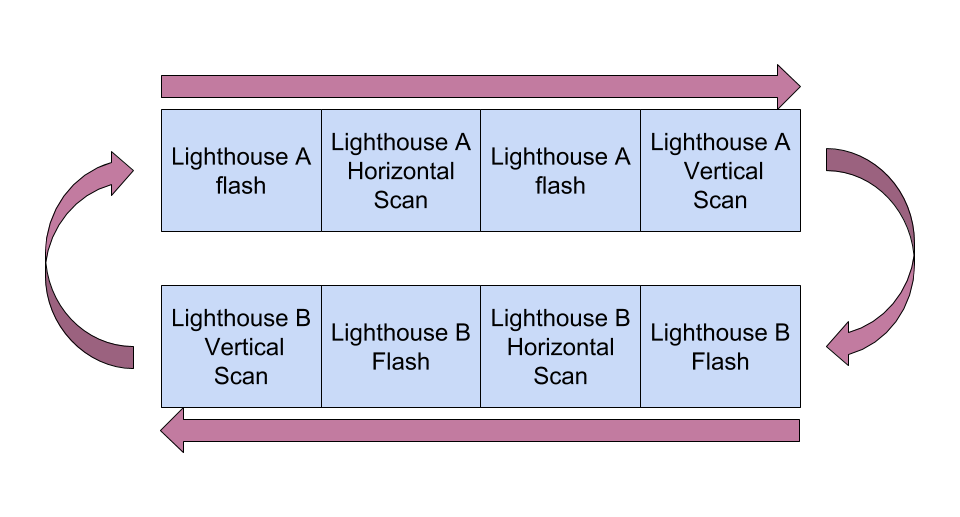
\includegraphics[scale = 0.24]{Image/LHLoop2.png}
  \caption{Representation of the periodic operation of the Lighthouse Tracking System (LTS). It begins with the flash emission of Lighthouse A, followed by a horizontal scan, another flash and a vertical scan. It then repeats the same pattern with Lighthouse B. Throughout the operation, the LTS will switch between Lighthouse A and B in the shown order.}
  \label{im:LHloop}
\end{figure}

Of course, in order to have a relevant sensor, the LTS needs to be fast. In fact, the sweeping plan will only scan half of a period, 180° then. This scanning takes $8.333 ms$, which means a full positioning is 4 time longer, since it needs 4 scan as seen in figure [\ref{im:LHloop}]. The flash are instantly emitted after the end of each sweeping, therefor, it doesn't make the positioning longer. In conclusion, the LTS can position an object every $33,350 ms$. \newline
However, to position an object, we need to look at the signal obtained from the photo-diode. An estimation of what we can expect from a photo-diode in a full period is given in figure [\ref{im:signal}].

The ratio of time obtained with the signal acquired with the photo-diode that is positioned on the object will be used to estimate 4 angles, that will be then used to compute the position of the object. The exact way the position is computed is given in section \ref{Sim}. \newline

\begin{figure}[h!]
  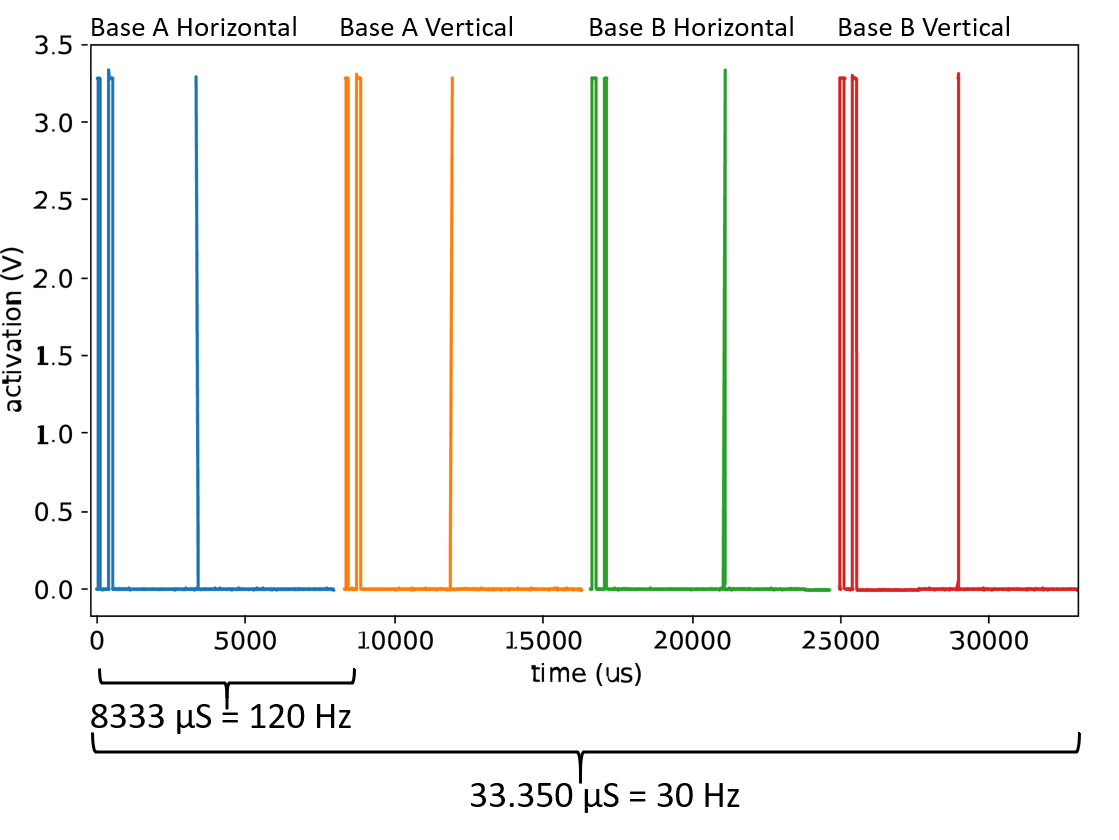
\includegraphics[scale = 0.28]{Image/signal.png}
  \caption{Estimation of the signal acquired by a photo-diode trough time in an optimal case. Each color represents one scanning for a total of 4 scanning for the full positioning. Before each sweeping plan, a flash is emitted by the lighthouse that can be seen at the beginning of each scanning plan. The other peak around the middle of each sweeping plan represents the moment it passes trough the photo-diode.}
  \label{im:signal}
\end{figure}

\subsection{Accelerometer} \label{Accel}

The LTS can position an object precisely every $33.350 ms$. It is fast, but not enough to be relevant if a fast movement occurs. Accelerometers are sensors that estimate the acceleration of an object at any time. It can be used as a real time positioning, since it allows to follow the movement in every direction. However, it gives no information about the position of the object. Also, because of the sensitivity and the error of any sensor, the estimated position, given that we know the position at the beginning, will be less and less accurate as times passes. This means, that unlike the LTS that gave accurate positions, the accelerometer cannot be used as 3D positioning system by itself. However, it brings useful information in real time about the movement undergone by the object. \newline
This leads to a need of fusing the LTS and the accelerometer in order to get ride of both disadvantages, i.e slowness and accuracy.

\section{Sensor Fusion} \label{SF}


The objective is to use the position given by the LTS that it is precise but with a slow rate and the data from the MicroElectroEechanical Systems (MEMS) sensors from the Inertial measurement unit (IMU) which are less precise but with a fast rate and process data fusion in order to have a faster rate and a good precision. Kalman filter is used to realize this data fusion. First, let's define the state system for a 3 degrees of freedom (DOF) object. The following explanations are adapted from \cite{caron2006gps}, but it is actually classical Kalman filter application. The state is :


\begin{equation}
\mathbf{X} = 
\begin{pmatrix}

x & \frac{dx}{dt} & \frac{d^2x}{dt^2} &
y & \frac{dy}{dt} & \frac{d^2y}{dt^2} &
z & \frac{dz}{dt} &  \frac{d^2z}{dt^2} 
\end{pmatrix} ^T
\end{equation}


note $dt$ the time elapsed since the last estimate. Then for an instant $k$ the estimate at $k+1$ is : 
\begin{equation}
\mathbf{X}(k+1) = A \mathbf{X}(k) +  \mathbf{w}(k)
\end{equation}
with $$\mathbf{A}=
\begin{pmatrix}
\begin{matrix}
\mathbf{F}
\end{matrix} &
\begin{matrix}
\mathbf{0_{3 \times 3}}
\end{matrix} &
\begin{matrix}
\mathbf{0_{3 \times 3}}
\end{matrix} \\
\begin{matrix}
\mathbf{0_{3 \times 3}}
\end{matrix} &
\begin{matrix}
\mathbf{F}
\end{matrix} &
\begin{matrix}
\mathbf{0_{3 \times 3}}
\end{matrix} \\
\begin{matrix}
\mathbf{0_{3 \times 3}}
\end{matrix} &
\begin{matrix}
\mathbf{0_{3 \times 3}}
\end{matrix} &
\begin{matrix}
\mathbf{F}
\end{matrix}
\end{pmatrix}$$
and $\mathbf{w}$ a zero mean white gaussian noise of assumed known covariance matrix $$ \mathbf{Q}(k) = E[ \mathbf{w}(k) \mathbf{w}(k)^T].$$ For  this 3 DOF object let's assume that $$\mathbf{F}=
\begin{pmatrix}
1 & dt & \frac{dt^2}{2} \\
0 & 1 & dt \\
0 & 0 & 1
\end{pmatrix}$$.  This model allows to estimate the next state from the actual state. Actually, that's obviously not enough to have a good estimation if $dt$ becomes too big or if the model can't rectify his state from a measurement. The Kalman filter can rectify the state from a measurement 
\begin{equation}
\mathbf{y}(k) = \mathbf{C} \mathbf{X}(k) + \mathbf{b}(k)
\end{equation} where $ \mathbf{C}$ is the measurement matrix and $\mathbf{b}$ is a white Gaussian observation noise with zero mean and with an assumed known covariance matrix
\begin{equation}
\mathbf{R}(k) = E[ \mathbf{b}(k) \mathbf{b}(k)^T]
\end{equation} The matrix $\mathbf{C}$ depends on the sensor which is feeding the kalman filter. For no measurement $\mathbf{C} = \mathbf{0_{3 \times 9}}$, for a measurement the matrix $\mathbf{C}$ have ones corresponding to each measurements. With this feeding from measurements the state can be evaluated as :
\begin{equation}
 \begin{matrix}
\hat{\mathbf{x}}(k|k) = \hat{\mathbf{x}}(k|k-1) +\\ \mathbf{K}(k)[\mathbf{y}(k)-\mathbf{C}\hat{\mathbf{x}}(k|k-1)]
\end{matrix}   
\end{equation}
 where $\mathbf{K}$ is the kalman gain. There is many integration of kalman filter on c++ language. In our case, $dt$ is not a constant. It depends on many factors like the final rate we want for kalaman estimation, also it depends on the measurement rate which is chaotic because of the using of several sensors and also because of the occlusions which destroy measurements. All this constraints can easily be manage in C++ by using an object which contains all the kalman filter information. Then, the algorithm can update the filter depends on the case : \\ - update without measurement \\ - update with positions measurements from the LEDs and light house system \\ - update with measurements from the IMU



\section{Framework and simulation} \label{FS}

To create the Graphic User Interface (GUI), we will use OpenFramework which is an OpenSource library allowing 3D modeling in C++ language. First, we will create the environment by defining the room and also a configuration panel. Then, we will show how the LTS and the accelerometer are simulated; and finally, the simulation of the sensor fusion.

\subsection{Framework} \label{Frame}

Our framework will be a room represented by a box whom dimensions can be modified with a control panel. In this room, there will be the object and the lighthouses. The Lighthouses will always be in the top opposite corner of the room, changing the dimension of the room will therefor change the position of the lighthouses. The position of the object can also be changed by the control panel. A representation of the simulation is given in figure [\ref{im:gui}].\newline

The dimension of the rooms are represented by pixels. The highest dimension of a room that we can use on OpenFramework is 2000 pixels per dimension. Above that, the simulation goes crazy and is unstable. A conventional small room is 5*5 meter square, which means that one pixel represent $0.25 cm$, which will be our precision.

\begin{figure}[h!]
  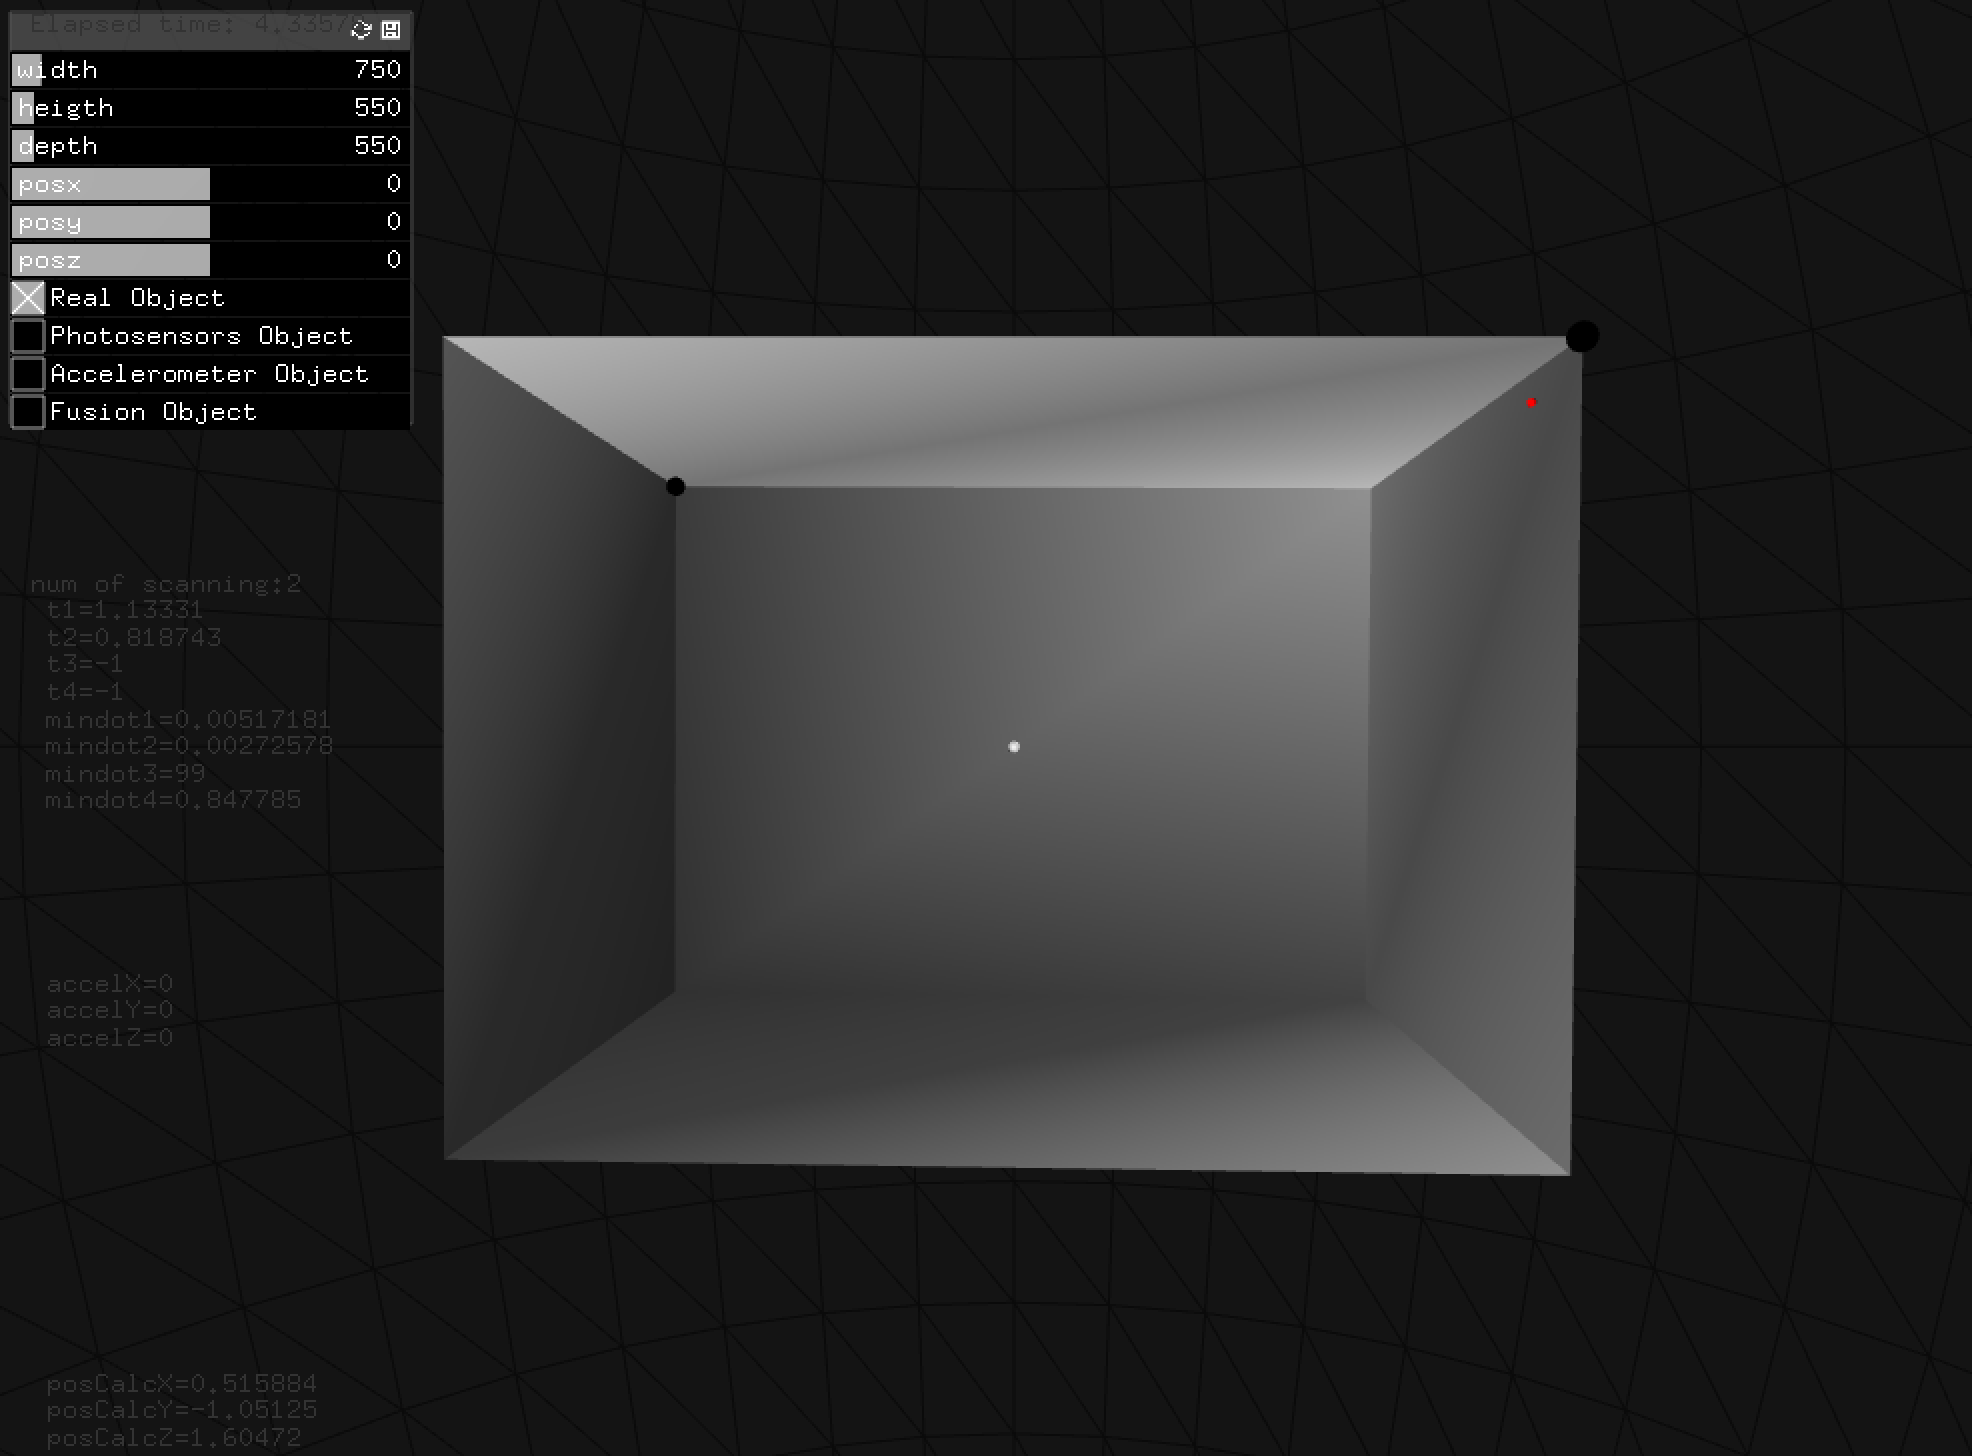
\includegraphics[scale = 0.24]{Image/gui3.png}
  \caption{Visualization of the room created Graphic User Interface (GUI) with OpenFrameworks. The object is in the center of the room, the lighthouses can be seen in it corners and the control panel is in the top left of the picture. The red sphere represent the normal to the plan vector of the sweeping plan. This vector is the one transforming the position of the emitting lighthouse to the red sphere.}
  \label{im:gui}
\end{figure}



%la piece defini en patron, panel de config...
\subsection{Sensors simulation} \label{Sim}
Since the framework is now well defined, we need to simulate the sensors, i.e the lighthouse and the accelerometer.
\subsubsection*{Simulation of the lighthouses}
In our framework, lighthouses are represented by spheres positioned in the top opposite corner of the room. The spheres are originally black, and become white whenever a flash occurs. The object is also represented by a white sphere in the middle of the room, but the position can be changed by the panel introduced in section \ref{Frame}.  \newline
The scanning of the room is defined by a normal vector of the sweeping plan (there are two normal vector for each plan, in our case, it doesn't matter which one we take) and the position of the emitting lighthouse, i.e a point. Two vectors are then used to obtain the moment when the sweeping plan passes through the object. One of them is the normal to plan vector that will rotate along side with the sweeping plan (and that can be seen in figure [\ref{im:gui}] as the red sphere); the other one is the Lighthouse-Object vector. This second vector is only known in the simulation, since we want to obtain the position of the object. However, this information is only used to obtain the moment when the sweeping plan passes through the object and is not used as a data as is. That moment is then obtained by looking at the scalar product between these two vectors. Indeed, when the scalar product is equal to zero, it means that the object is currently in the sweeping plan. In our simulation, that moment is obtained when the scalar product is the smallest (since it is hard to obtain the moment when it's exactly equal to 0). Figure [\ref{im:scalar}] shows an example of the scalar product obtained from one sweeping.

\begin{figure}[h!]
  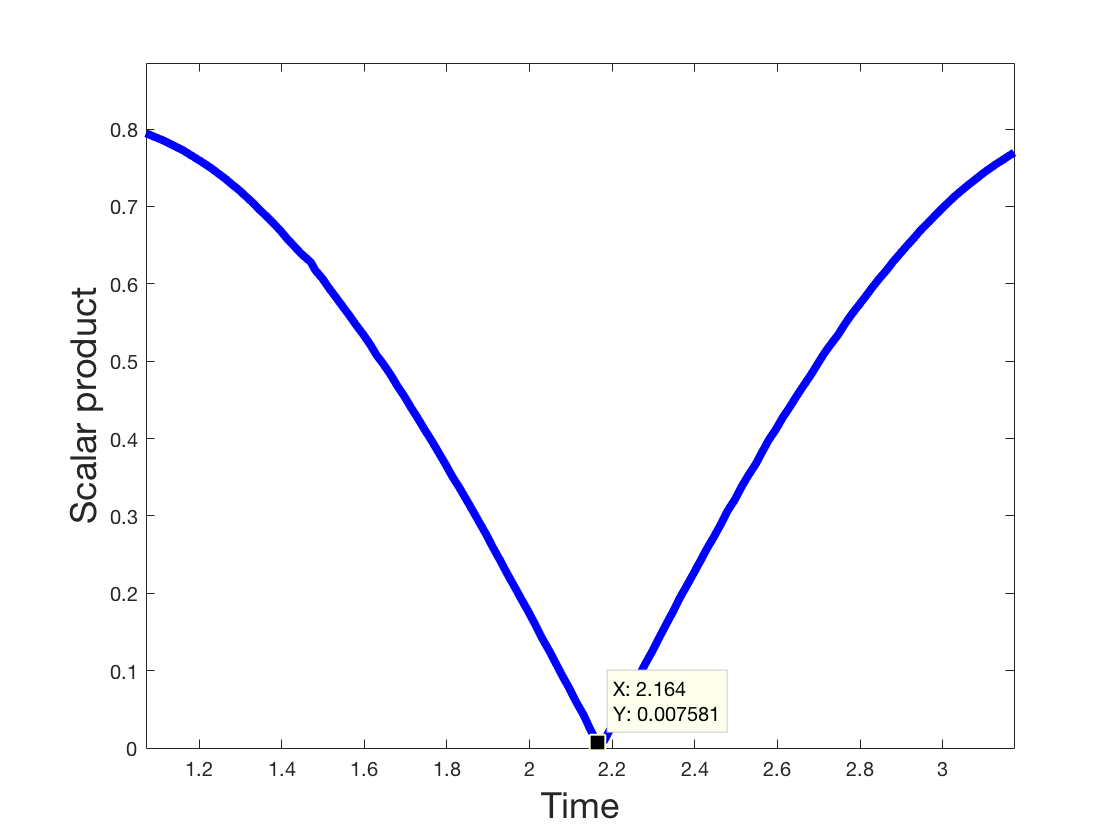
\includegraphics[scale = 0.21]{Image/scalaire.png}
  \caption{Evolution of the scalar product between the Lighthouse-object vector and the normal to the plan vector through time. We consider that the time when this value is the lowest as the moment the sweeping plan passes through the object. In this situation, the object is in the middle of the room.}
  \label{im:scalar}
\end{figure}

The obtaining of the time after the four sweeping will allows us to obtain the four angles as wanted. We then use spherical coordinate to obtain two Lighthouse-Object vector from the two lighthouses. These vectors combined with their respective lighthouses will lead to the obtaning of the lines, and the intersection of the two lines will be the position of the object. \newline
However, it is really rare that two lines intersect each other in a 3D space. So we need an approximation of that point and one method consist of finding a third line perpendicularly intersecting the two first lines and then consider the point between the two intersected point of the lines as the position of the object. Figure [\ref{im:intersection}] illustrates better how this point is obtained.

\begin{figure}[h!]
  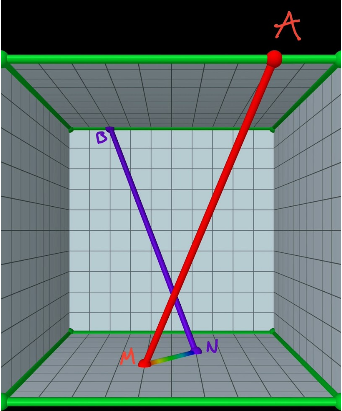
\includegraphics[scale = 0.92]{Image/interscetion.png}
  \caption{Illustration of the method used to compute the closest approximation of the intersection of two lines in 3D space. In our situation, $A$ and $B$ are the lighthouses, and the object will be in the middle the $MN$ segment}
  \label{im:intersection}
\end{figure}


\subsubsection*{Simulation of the accelerometer}
The values obtained from the accelerometers are obtained by derivating twice the position of the object. We add an error at that moment and then move the object according to the value obtained by integrating it twice.



\subsection{Fusion} \label{Fusion} 

We use Eigen library to implement the Kalman Filter. During the simulation, Kalman filter is first initialized with values equal to zero. Every time we obtain new values from the accelerometer or from the LTS, we update the Kalman filters. It means we update: the command Matrix $C$ that indicates what type of measurements do we have (position, speed or acceleration), the elapsed time from the last update and the noise covariance matrix. \newline
The noise covariance Matrix of the position acquired from the LTS is obtained from the mean of 20 tests made in the simulation. It values can be seen in the matrix below.

$$\begin{pmatrix}
0.5901 & -0.0280 & 0.3103 \\
-0.0280 & 0.4582 & -0.0732 \\\
0.3103 & -0.0732 & 0.4489
\end{pmatrix}$$

The noise covariance matrix is harder to estimate because of its dependence with the time. We decided to define it as an identity Matrix multiplied by 1000 to reduce its importance regarding to the measurements of the lighthouse.
\section{Results} \label{Res}
This section shows the results obtained from the simulation. Figure [\ref{im:visu}] shows 4 balls, each representing one position computed by the simulator. White is the real position, blue the one obtained only with the LTS, red the position estimated from the accelerometters only and green is the position of obtained from the fusion
\begin{figure}[h!]
  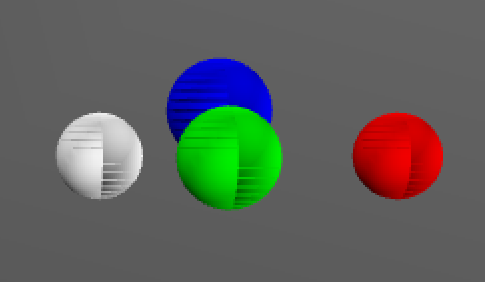
\includegraphics[scale = 0.65]{Image/Visulaisation.png}
  \caption{Closer representation of the object and their estimated position in the simulation. The white ball represent the real position, the blue one represent the position estimated from the Lighthouse Tracking System, the red one represents the position of the object estimated with the accelerometter only and the green ball represents the position estimated from the sensor fusion.}
  \label{im:visu}
\end{figure}

What is interesting to look at is the evolution of the position of the object trough time. Figure [\ref{im:res}] shows  the position of the object and with each position estimated.
\begin{figure}[h!]
  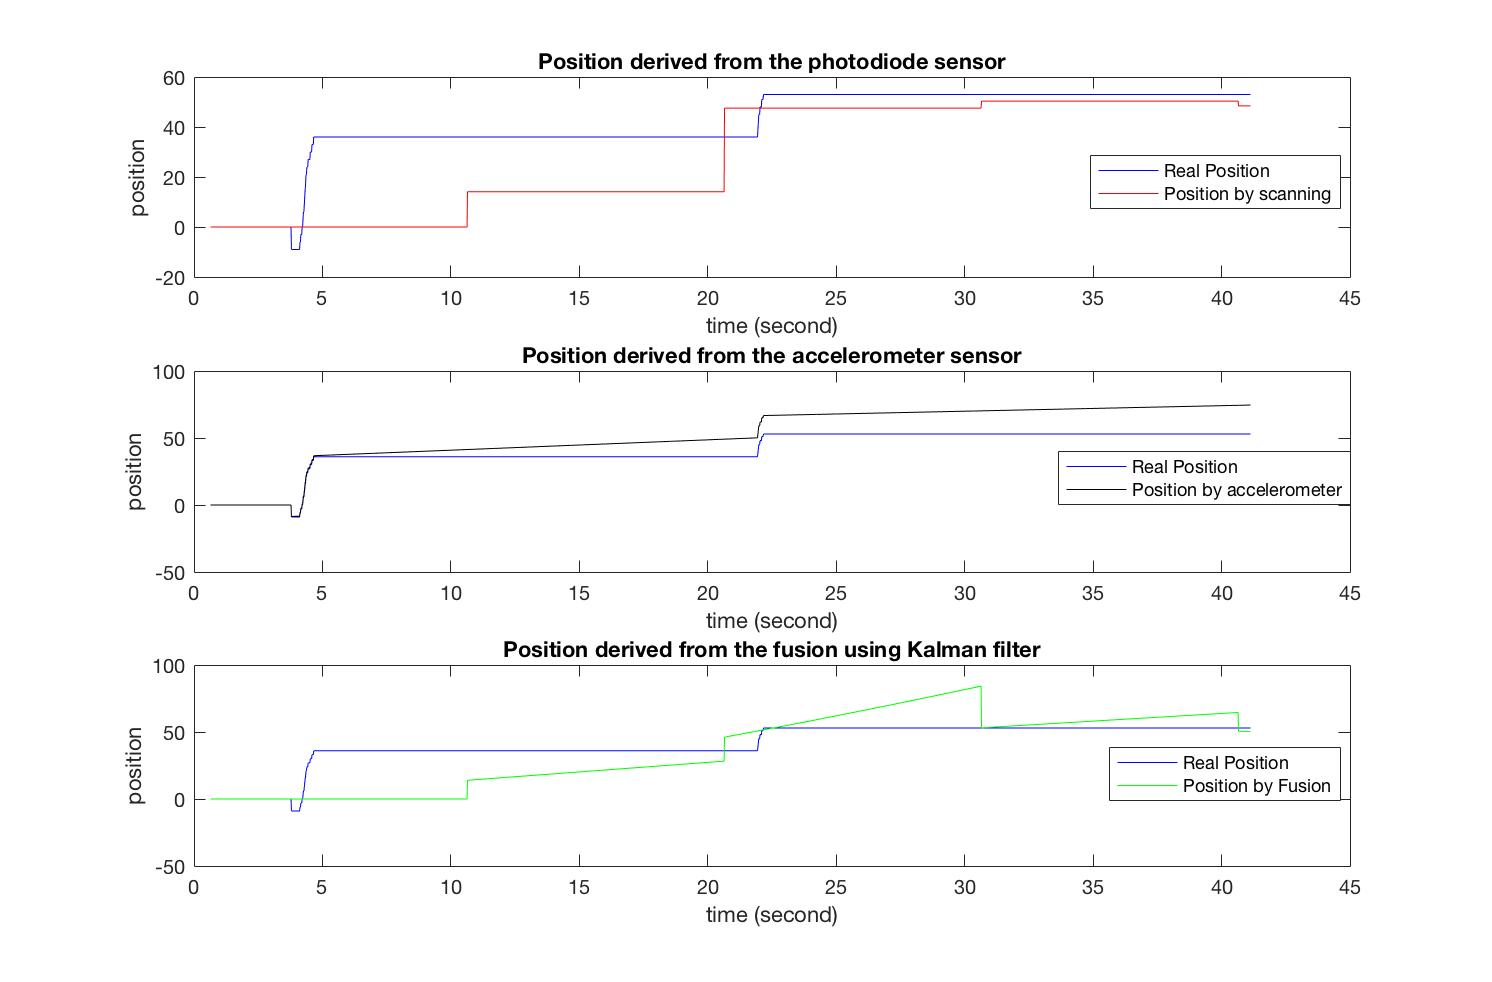
\includegraphics[scale = 0.15]{Image/ResultKalman.jpg}
  \caption{Evolution of the position of the objects through time. Each plot compares the real position with one of the position estimator.}
  \label{im:res}
\end{figure}

As it can be seen, the LTS is slowly updated but pretty precise, the accellerometter follows the object faster but tends to increase its error with time. The fusion gives the fastest and the most precise values, since it is updated faster and eliminate the accumulation of error of the accellerometter.
% The following two commands are all you need in the
% initial runs of your .tex file to
% produce the bibliography for the citations in your paper.
\bibliographystyle{abbrv}
\bibliography{vldb_sample}  % vldb_sample.bib is the name of the Bibliography in this case
% You must have a proper ".bib" file
%  and remember to run:
% latex bibtex latex latex
% to resolve all references



%APPENDIX is optional.
% ****************** APPENDIX **************************************
% Example of an appendix; typically would start on a new page
%pagebreak



\end{document}
